\chapter{Background}
Everyone knows what is WP and how to use it in a basic way but there lots of functionality
there a lot of people ignore, starting from the fact that everyone can edit a page and all the
versions are publicly available. Anyone with a browser can see and compare all the edits in a
wikipedia page, but for developers there exist much powerful resources such as big Datasets 
containing a lot more informations.  

\section{History Exploration}
There are several tools anyone can use to explore revision history: 
\begin{wrapfigure}[12]{r}{0.5\textwidth}[h]
    \centering
    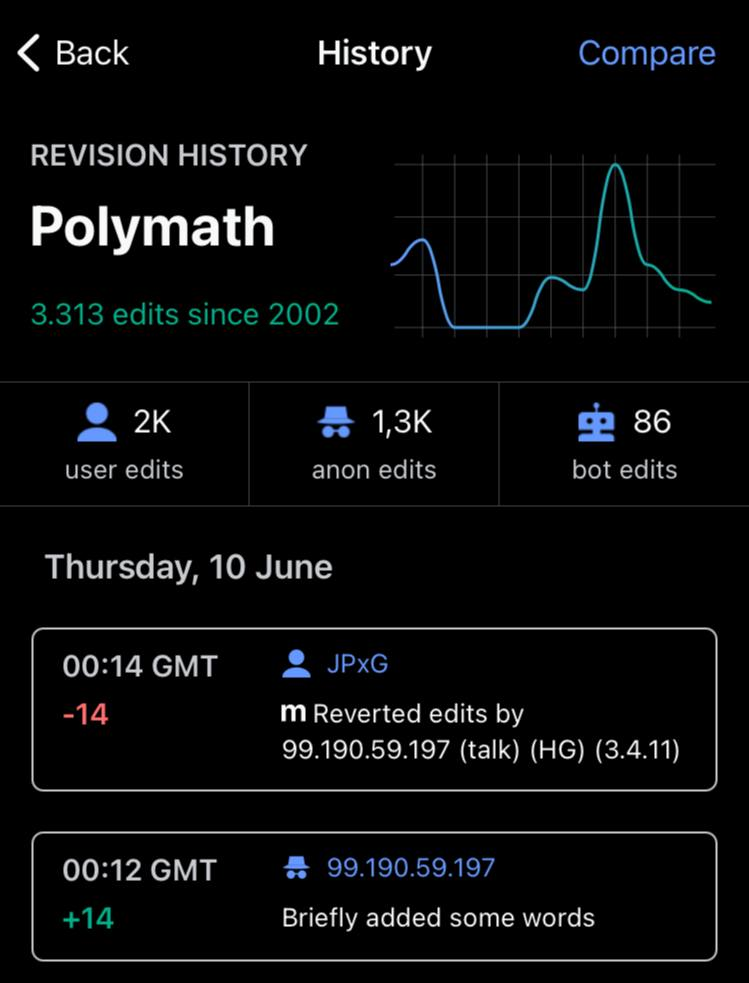
\includegraphics[width=0.35\textwidth]{./chapters/02/assets/mobile_history.jpg}
    \caption{mobile interactive visualization of the history}
    \label{fig:mobilehistory}
\end{wrapfigure}

\begin{itemize}
    \item Mobile application: this resource is only avaiable in the mobile application and gives
        some statistics about the edits of the page like the total number of edits 
    \item History page: it is possibile to compare two edits with an interactive tool which show the
        trend of the pages edit : for each edit matches a bar indicating the number of bytes added or
        removed by the revision 
\end{itemize}



\begin{figure}[h]
    \centering
    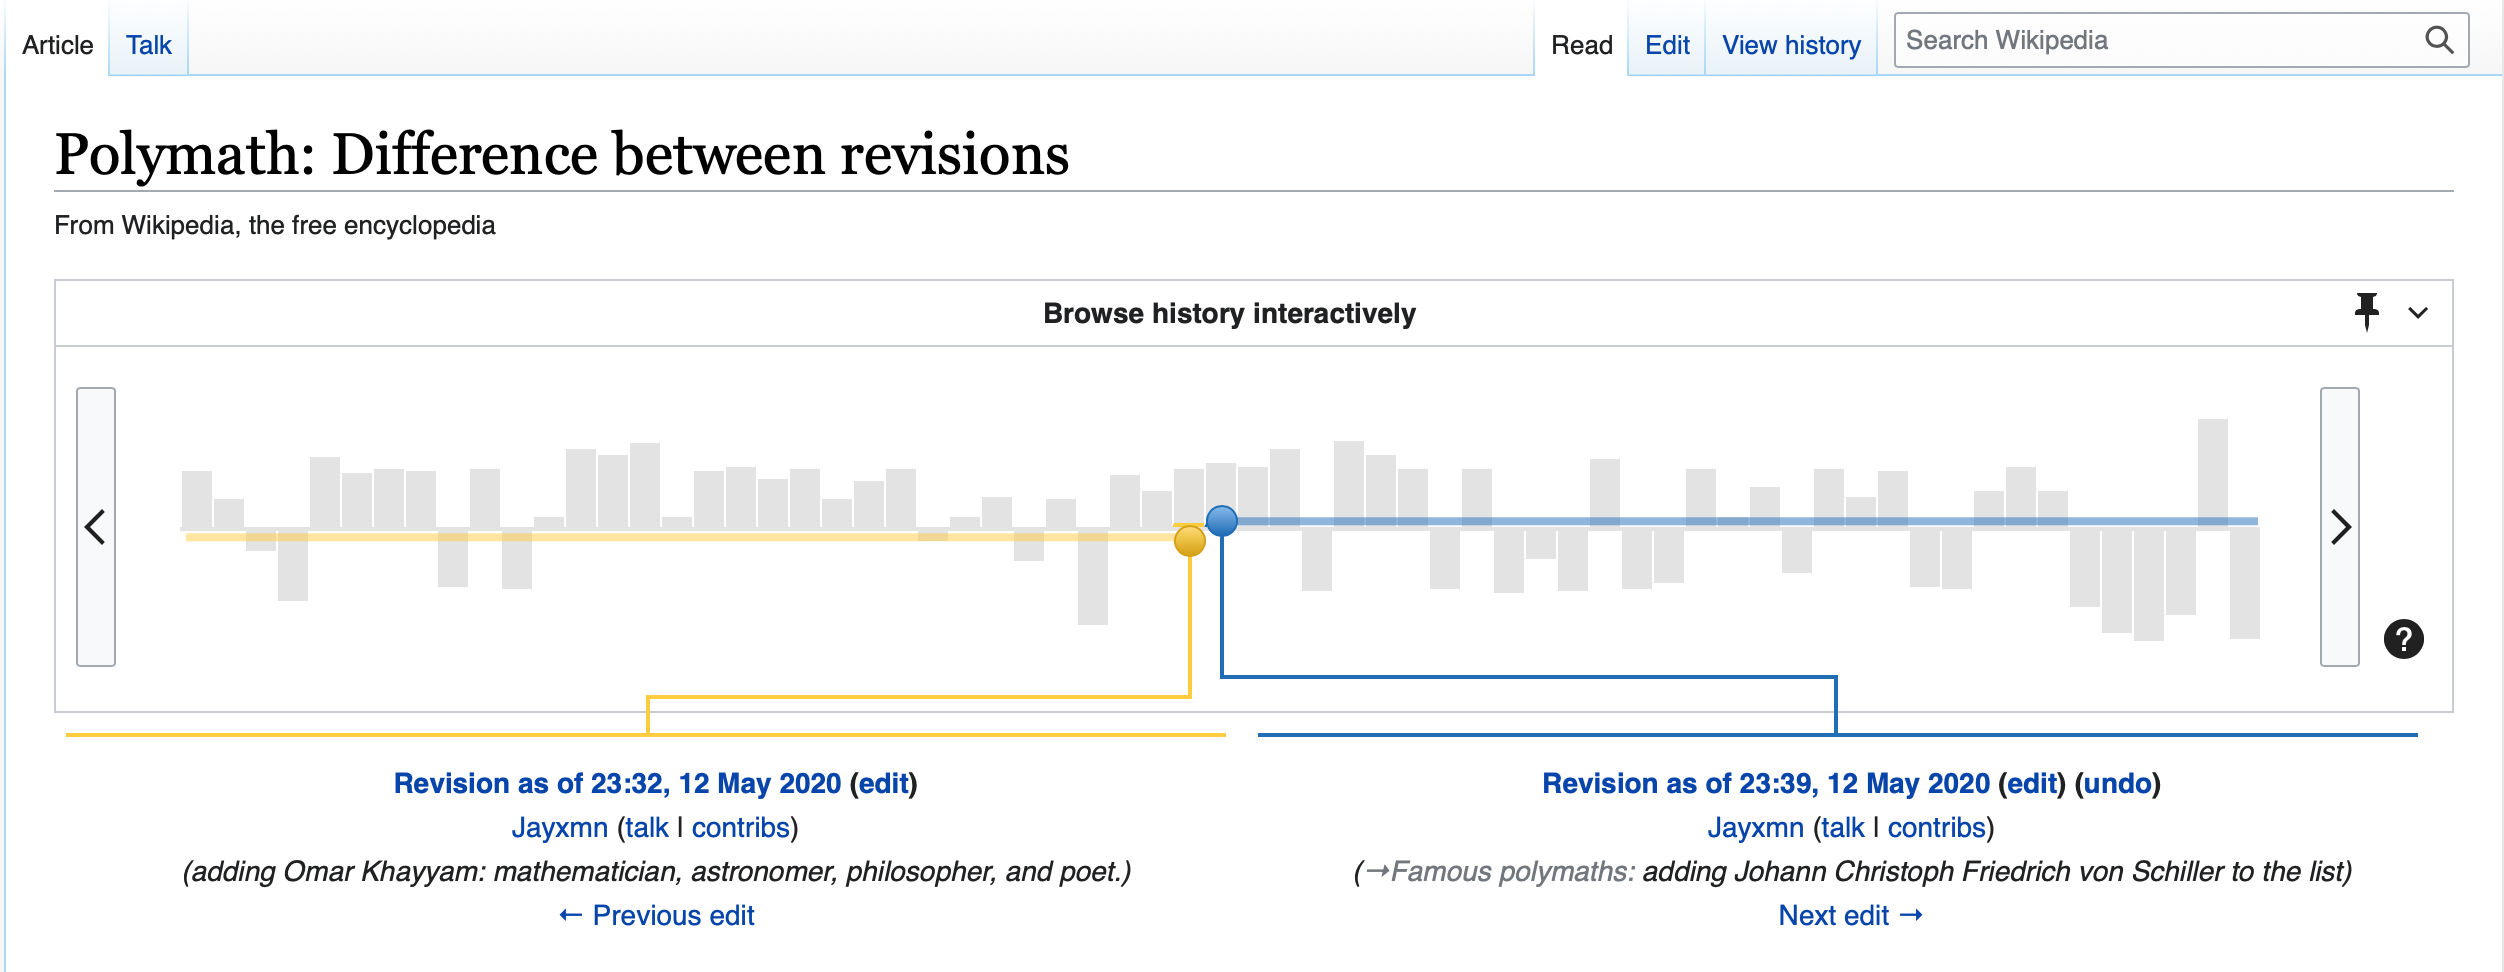
\includegraphics[width=1\textwidth]{./chapters/02/assets/history.png}
    \caption{interactive visualization of the history}
    \label{fig:history}
\end{figure}


\section{Dataset}
There are two datasets that store info about WP edits made available from the WikiMedia Foundation
\begin{itemize}
    \item MediaWiki History
    \item MediaWiki History Dumps
\end{itemize}

The only difference beyond the format ( XML the first one TSV the second) is that the first one also
contains the content of the page. The dataset used in this study is the MediaWiki History Dumps.

\subsection{MediaWiki History Dumps}
The dataset used contains information about all events that has happened in WP since 2001. There are 3 types
of events:
\begin{itemize}
    \item page: when a page is created, moved, restored, merged ,deleted 
    \item user: when a user is created, renamed, blocked, changed the rights 
    \item revision: when a page is edited 
\end{itemize}

In this analysis the only revision events are interesting, there are 68 fields divided in different
 sections: the first one with general info of the revision like timestamp and comment, a section
 with info about the user who made the revision, one for the page involved, and the last one with
 more specific information about the revision



\begin{table}[H]
    \centering
    \ra{1.2}
    \begin{tabularx}{\columnwidth}{@{}Xccccc@{}}
        \midrule
        \textbf{id} & \textbf{text} & \textbf{groups} & \textbf{is\_anonymous} & \textbf{registration} & \textbf{revision\_count}\\ \toprule
        42081 & Checco & autopatrolled & False & 2006-02-10 14:52:44.0 & 10479 \\

         \bottomrule
    \end{tabularx}
    \caption{data about user that made the revision}
\end{table}


\begin{table}[H]
    \centering
    \ra{1.2}
    \begin{tabularx}{\columnwidth}{@{}Xccc@{}}
        \midrule
        \textbf{id} & \textbf{title} & \textbf{namespace} & \textbf{revision\_count} \\ \toprule
        116530 & Pino\_Rauti & 0 &  195 
        \\

         \bottomrule
    \end{tabularx}
    \caption{data about the page where the revision is made}
\end{table}

\begin{table}[H]
    \centering
    \ra{1.2}
    \begin{tabularx}{\columnwidth}{@{}Xcccc@{}}
        \midrule
        \textbf{id} & \textbf{parent\_id} & \textbf{is\_reverted} & \textbf{reverter\_id} & \textbf{is\_reverter} \\ \toprule
        73507165 & 73506955 & True &  73511400 & False 
        \\

         \bottomrule
    \end{tabularx}
    \caption{data about the revision}
\end{table}


\section{Definitions}
It is useful to define some terms that will be used different times

\newtheorem{definition}{definition}
\begin{definition}
    (Revert) On Wikipedia, reverting means undoing or otherwise negating the effects of one or more edits,
    which results in the page (or a part of it) being restored to a previous version. 
\end{definition}

\begin{definition}
    (Revert chain) On a Wikipedia page, a revert chain happens when an edit which reverts an edit is in turn reverted.
\end{definition}

\begin{definition}
    (Mutual revert) A “mutual revert” is recognized if a pair of editors (x, y) is observed once with x and once with y as the reverter~\cite{Yasseri2014}.
\end{definition}

\begin{definition}
    (Editor weight) The weight of an editor x is defined as the number of edits N performed by him or her.
\end{definition}

\begin{definition}
    (Mutual revert weight) The weight of a mutually reverting pair MW is defined as the minimum of the weights of the two editors.
\end{definition}

\begin{definition}
    (Chain weight) The weight of a revert chain CW is defined as the minimum of the weights of the editors involved in the chain.
\end{definition}


\section{Metrics}
Two complex controversiality metrics have been computed in this study: the first one,M, is the state of the
art metric introduced by Yasseri \textit{et al.} which give us a score of the controversiality of the page
based on mutual reverts. The second one that we designed, called G, is very similar to M, but
instead of using mutual reverts it uses revert chains to evaluate the controversy of the page  

\subsection{M}
The controversiality M of an article is defined by summing the weights of all mutually reverting
editor pairs, excluding the topmost pair, and multiplying this number by the total number of editors
E involved in the article.

\begin{equation}
    M = E   \sum_{all\ mutual\ reverts} MW
\end{equation}

\subsection{G}
The controversiality G of an article or user is defined by summing the weights off all the chains
there are in a page or a user is involved, and multiplying by the total number of editors N involved in at least one chain.

\begin{equation}
    G = N \sum_{all\ revert\ chains} CW
\end{equation}




